%!TEX root = ../../main.tex
\subsection{Blockchain}
\label{ch:approach:intro:blockchain}
Blockchain-based distributed database systems are emerging technologies that aim to provide users with the necessary tools to perform tasks and computations without the assistance of an intermediate entity, to build self-trust systems where rules are agreed upon beforehand, and to create the basis for an ecosystem th can be used by everyone. Moreover, users may interact democratically and be confident that committed transactions will be immutable, truthful, and irrefutable\footnote{Bitcoin is the first and most famous example of a worldwide distributed blockchain system. 
}.

In its nature, a Blockchain is basically an immutable unbreakable data storage structure. It consists of a set of components that allow a set of data to be stored in small blocks and be linked by a Hash function to the Hash of its predecessor, forming a chain of blocks that all all the holding systems can verify and validate. This chain of blocks form a \emph{Merkle Tree} structure; when the data inside any of the block changed by malicious users,  the rest of the chain will not be approved by the community, thus resulting on a waste of resources and time. This happens because the hash of the \emph{Merkle tree} will change and be different from the rest of the other nodes.

\begin{figure}[!h]
    \centering
    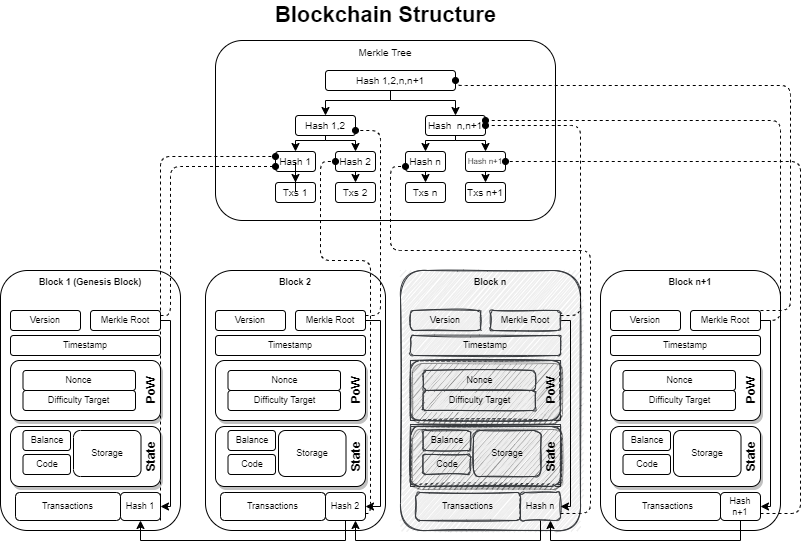
\includegraphics[width=180mm]{img/BlockchainStructure.png}
    \caption{Structure of a \ac{PoW} Blockchain ledger}
    \label{fig:BlockchainStructure}
\end{figure}

\subsection{Blockchain Ledger}
Figure \ref{fig:BlockchainStructure} shows the main components of a Blockchain structure which form the Ledger. This basic components are generated and validated by the different nodes in the System and later allow other users to interact and submit transactions to it. Depending of the type of blockchain different consensus mechanisms are generated in order to insert and validate the transactions block by block. 
The components of the ledger are:
\subsubsection{Block}
Represents a set of stored transactions submitted by different users and approved by node validators. To be able to insert data into a single block, certain rules have to apply: 
\begin{itemize}
    \item A user connected to the system and willing to insert data (submit a transaction) needs to prove its identity with a public and private key, which will allow him to interact with its asset in order to update the ledger by sensing or receiving (update or submit). Once the user and its ownership are properly identified and approved respectively, the transaction enters in a "data cache" where other transactions are waiting to be submitted in the ledger. There are several ways data can be validated and approved to be inserted into the ledger, but most commonly public Blockchains will request a transaction fee (paid in tokens) to commit the transaction. The fee allows the system to function as the machines in charge of maintaining and approving the transactions receive such value in exchange of the resources they use. Depending on the amount paid in the fee, the transaction will take or not priority to be inserted in the next block. Once the block reaches a certain size or time, it is generated, hashes and send to other peers.
\end{itemize}

\subsubsection{Version}
Indicates the version that the particular block uses. There are three types of Blockchain versions.

\begin{itemize}
    \item \emph{Version 1.0 (cryptocurrency)} ). It used a public ledger to store the data.
    \item \emph{Version 2.0 (Smart Contracts)} ). Indicates that embedded source code in the block has been executed for the generation of the block.
    \item \emph{Version 3.0 (\ac{DAPP}s )}. It is used to create a decentralized structure, such as the Tor Browser.
    \item \emph{Version 4.0 (Blockchain for Industry)}. Used to create a scalable, affordable blockchain network so that more people can make use of it.
\end{itemize}
 
\subsubsection{Timestamp}
Used as proof that the particular block is used at what instance of a time. It is also used as a parameter to verify the authenticity of a block.

\subsubsection{Consensus}
\label{consensus}
A consensus is a fault-tolerant mechanism used to achieve agreement on a single data value or a single state of the network among distributed processes or multi-agent systems. It allows all parties to participate democratically and enable equal rights to validate and insert data in the Blockchain.

There are different consensus mechanisms\cite{BlockchainConsensus:online}: 
\begin{itemize}
    \item \emph{\ac{PoW}}
    One party proves to another which verifies that a particular computational effort has been expended. Subsequently, verification can be accomplished with minimal effort on the part of the verifying party. By requiring some work from a service requester, such as processing time by a computer, it was initially conceived to deter denial-of-service attacks and other forms of network abuse. In Bitcoin, it is used as a consensus mechanism for a permissionless decentralized network in which miners compete to append blocks and issue new currency with a success probability proportional to the computational effort expended.  A key characteristic of proof-of-work schemes is their asymmetry\footnote{The work (computation) that must be moderately complex, yet feasible by a computer (prover) but simple to verify by the service provider (verifier)}. Its design contains a built-in incentive structure that rewards validators by allocating computational capacity to the network with value in the form of money.  \ac{PoW} algorithms aim to deter data manipulation by establishing considerable energy and hardware-control requirements, thus expending large amounts of resources in the process.
    
    \item \emph{\ac{PoS}}
    This method avoids the computational cost associated with proof-of-work schemes by selecting validators based on their holdings of the associated cryptocurrency. The validators are rewarded for adding transactions to the block. PoS secures a system by requiring validators to possess some blockchain tokens to mount an attack. Because PoW does not require complex mathematical calculations, it is more energy-efficient.
    
    \item \emph{\ac{PoET}}
    It is commonly used on a permissioned Blockchain. First, every node in the system must be identifiable and accepted into the network. Then, a standard certificate authority validates them. With PoET, the “timer” is different for each node. Each participant in the network is assigned a random amount of time to wait. The first participant to finish waiting gets to commit the following block to the blockchain.
    
    \item \emph{\ac{PoA}}
    It is a spin on \ac{PoS} consensus that addresses the risk of how participants in a network can value a stake. the consensus stakes the actual identities of the nodes in the system and aligns incentives by placing social capital at risk. A greater incentive is to act in the network's best interest if more of its net worth is lodged in a node, therefore  wealthier participants could go \ac{AWOL} as they can eat any financial loss they would receive for doing so. There also exist validation nodes,  which stake their reputation on the network. As compensation, validators are the only nodes allowed to validate blocks. By identifying validators, \ac{PoA} consensus becomes inherently centralized and best suited for private Blockchains and consortiums, such as a group of banks or insurance companies.

    \item \emph{\ac{BFT}}
    Allows distributed system to reach consensus (agreement on the same value) even when some of the nodes in the network fail to respond or respond with incorrect information. The objective is to safeguard against the system failures by employing collective decision making when it is both correct and misleading. It aims to reduce influence of the faulty nodes. \ac{BFT} is derived from Byzantine Generals’ Problem\footnote{The Byzantine Generals Problem is a term etched from the computer science description of a situation where involved parties must agree on a single strategy in order to avoid complete failure, but where some of the involved parties are corrupt and disseminating false information or are otherwise unreliable.}.
    
    
    \item \emph{\ac{PBFT}}
    Designed to work efficiently in asynchronous systems. It is optimized for low overhead time. Its goal was to solve many problems associated with already available \ac{BFT} solutions. It has a primary node and secondary nodes. These nodes work together to reach a consensus, making this system one of the solutions to the Byzantine Generals Problem. The maximum number of faulty/malicious nodes cannot be equal to or greater than one-third of the total nodes in the system.

    \item \emph{\ac{DAG}}
    A directed graph is a \ac{DAG} if and only if it can be topologically ordered, by arranging the vertices as a linear ordering that is consistent with all edge directions. To send a transaction, a node must validate two or more transactions that already took place. As more transactions are sent through the network, that system of checks and balances strengthens. The flow of data through this model allows the reduction of transactional fees, since they are approved as users contribute to the security of the network by confirming past transactions.

\end{itemize}


\subsubsection{\ac{Nonce}}
Is an arbitrary number that can be used just once in a cryptographic communication. Such number will never be repeated, and is the result that a machine has to come across in order to be the first on providing the hash of that number.

\subsubsection{Difficulty Target}
Is a measure of how difficult it is to mine a block in a blockchain for a particular cryptocurrency with \ac{PoW} consensus. A high cryptocurrency difficulty means it takes additional computing power to verify transactions entered on a blockchain—a process called mining.
\subsubsection{State}
It is a pointer that systems of the blockchain system independently hold their own copy of the blockchain, and the current known "state" is calculated by processing each transaction in order as it appears in the ledger. Transactions are bundled and delivered to each node in the form of a block. As new transactions are distributed throughout the network, they are independently verified and "processed" by each node.
\subsubsection{Transactions}
Continuously set of data being created or updated in the ledger. Contains relevant information about the digital assets or smart contract instructions to operate and change the ledger.
\subsubsection{Hash}
It is the process of transforming any given key or a string of characters into a new value through the process of hashing. Shorter, fixed-length values can be represented by keys that enable finding and using the original data. A hash function generates new values according to a mathematical algorithm.. To prevent the conversion of hash back into the original key, a good hash always uses a one-way hashing algorithm.

\subsubsection{Merkle Tree}

Hash trees or Merkle trees are trees in which every leaf (node) is labelled with a cryptographic hash of a data block. The cryptographic hash of each inner node's label is included in its label. It allows efficient and secure verification of the contents of large data structures. Hash trees are a combination of hash lists and hash chains.


\subsection{Additional generalities}
All these components are basic to most of the Blockchain systems, regarding how nodes are assembled into the network depend mostly on the consensus mechanism adopted. for the purpose of this work the consensus aforementioned were deeply studied and incorporated in the proposal solution as it will be shown in the next sections.